% Options for packages loaded elsewhere
\PassOptionsToPackage{unicode}{hyperref}
\PassOptionsToPackage{hyphens}{url}
%
\documentclass[
]{article}
\usepackage{amsmath,amssymb}
\usepackage{iftex}
\ifPDFTeX
  \usepackage[T1]{fontenc}
  \usepackage[utf8]{inputenc}
  \usepackage{textcomp} % provide euro and other symbols
\else % if luatex or xetex
  \usepackage{unicode-math} % this also loads fontspec
  \defaultfontfeatures{Scale=MatchLowercase}
  \defaultfontfeatures[\rmfamily]{Ligatures=TeX,Scale=1}
\fi
\usepackage{lmodern}
\ifPDFTeX\else
  % xetex/luatex font selection
\fi
% Use upquote if available, for straight quotes in verbatim environments
\IfFileExists{upquote.sty}{\usepackage{upquote}}{}
\IfFileExists{microtype.sty}{% use microtype if available
  \usepackage[]{microtype}
  \UseMicrotypeSet[protrusion]{basicmath} % disable protrusion for tt fonts
}{}
\makeatletter
\@ifundefined{KOMAClassName}{% if non-KOMA class
  \IfFileExists{parskip.sty}{%
    \usepackage{parskip}
  }{% else
    \setlength{\parindent}{0pt}
    \setlength{\parskip}{6pt plus 2pt minus 1pt}}
}{% if KOMA class
  \KOMAoptions{parskip=half}}
\makeatother
\usepackage{xcolor}
\usepackage[margin=1in]{geometry}
\usepackage{color}
\usepackage{fancyvrb}
\newcommand{\VerbBar}{|}
\newcommand{\VERB}{\Verb[commandchars=\\\{\}]}
\DefineVerbatimEnvironment{Highlighting}{Verbatim}{commandchars=\\\{\}}
% Add ',fontsize=\small' for more characters per line
\usepackage{framed}
\definecolor{shadecolor}{RGB}{248,248,248}
\newenvironment{Shaded}{\begin{snugshade}}{\end{snugshade}}
\newcommand{\AlertTok}[1]{\textcolor[rgb]{0.94,0.16,0.16}{#1}}
\newcommand{\AnnotationTok}[1]{\textcolor[rgb]{0.56,0.35,0.01}{\textbf{\textit{#1}}}}
\newcommand{\AttributeTok}[1]{\textcolor[rgb]{0.13,0.29,0.53}{#1}}
\newcommand{\BaseNTok}[1]{\textcolor[rgb]{0.00,0.00,0.81}{#1}}
\newcommand{\BuiltInTok}[1]{#1}
\newcommand{\CharTok}[1]{\textcolor[rgb]{0.31,0.60,0.02}{#1}}
\newcommand{\CommentTok}[1]{\textcolor[rgb]{0.56,0.35,0.01}{\textit{#1}}}
\newcommand{\CommentVarTok}[1]{\textcolor[rgb]{0.56,0.35,0.01}{\textbf{\textit{#1}}}}
\newcommand{\ConstantTok}[1]{\textcolor[rgb]{0.56,0.35,0.01}{#1}}
\newcommand{\ControlFlowTok}[1]{\textcolor[rgb]{0.13,0.29,0.53}{\textbf{#1}}}
\newcommand{\DataTypeTok}[1]{\textcolor[rgb]{0.13,0.29,0.53}{#1}}
\newcommand{\DecValTok}[1]{\textcolor[rgb]{0.00,0.00,0.81}{#1}}
\newcommand{\DocumentationTok}[1]{\textcolor[rgb]{0.56,0.35,0.01}{\textbf{\textit{#1}}}}
\newcommand{\ErrorTok}[1]{\textcolor[rgb]{0.64,0.00,0.00}{\textbf{#1}}}
\newcommand{\ExtensionTok}[1]{#1}
\newcommand{\FloatTok}[1]{\textcolor[rgb]{0.00,0.00,0.81}{#1}}
\newcommand{\FunctionTok}[1]{\textcolor[rgb]{0.13,0.29,0.53}{\textbf{#1}}}
\newcommand{\ImportTok}[1]{#1}
\newcommand{\InformationTok}[1]{\textcolor[rgb]{0.56,0.35,0.01}{\textbf{\textit{#1}}}}
\newcommand{\KeywordTok}[1]{\textcolor[rgb]{0.13,0.29,0.53}{\textbf{#1}}}
\newcommand{\NormalTok}[1]{#1}
\newcommand{\OperatorTok}[1]{\textcolor[rgb]{0.81,0.36,0.00}{\textbf{#1}}}
\newcommand{\OtherTok}[1]{\textcolor[rgb]{0.56,0.35,0.01}{#1}}
\newcommand{\PreprocessorTok}[1]{\textcolor[rgb]{0.56,0.35,0.01}{\textit{#1}}}
\newcommand{\RegionMarkerTok}[1]{#1}
\newcommand{\SpecialCharTok}[1]{\textcolor[rgb]{0.81,0.36,0.00}{\textbf{#1}}}
\newcommand{\SpecialStringTok}[1]{\textcolor[rgb]{0.31,0.60,0.02}{#1}}
\newcommand{\StringTok}[1]{\textcolor[rgb]{0.31,0.60,0.02}{#1}}
\newcommand{\VariableTok}[1]{\textcolor[rgb]{0.00,0.00,0.00}{#1}}
\newcommand{\VerbatimStringTok}[1]{\textcolor[rgb]{0.31,0.60,0.02}{#1}}
\newcommand{\WarningTok}[1]{\textcolor[rgb]{0.56,0.35,0.01}{\textbf{\textit{#1}}}}
\usepackage{graphicx}
\makeatletter
\def\maxwidth{\ifdim\Gin@nat@width>\linewidth\linewidth\else\Gin@nat@width\fi}
\def\maxheight{\ifdim\Gin@nat@height>\textheight\textheight\else\Gin@nat@height\fi}
\makeatother
% Scale images if necessary, so that they will not overflow the page
% margins by default, and it is still possible to overwrite the defaults
% using explicit options in \includegraphics[width, height, ...]{}
\setkeys{Gin}{width=\maxwidth,height=\maxheight,keepaspectratio}
% Set default figure placement to htbp
\makeatletter
\def\fps@figure{htbp}
\makeatother
\setlength{\emergencystretch}{3em} % prevent overfull lines
\providecommand{\tightlist}{%
  \setlength{\itemsep}{0pt}\setlength{\parskip}{0pt}}
\setcounter{secnumdepth}{-\maxdimen} % remove section numbering
\ifLuaTeX
  \usepackage{selnolig}  % disable illegal ligatures
\fi
\IfFileExists{bookmark.sty}{\usepackage{bookmark}}{\usepackage{hyperref}}
\IfFileExists{xurl.sty}{\usepackage{xurl}}{} % add URL line breaks if available
\urlstyle{same}
\hypersetup{
  pdftitle={Quantitative Methods - Computer Lab 0},
  pdfauthor={Ralf Becker},
  hidelinks,
  pdfcreator={LaTeX via pandoc}}

\title{Quantitative Methods - Computer Lab 0}
\author{Ralf Becker}
\date{1 February 2022}

\begin{document}
\maketitle

\hypertarget{learning-outcomes}{%
\section{Learning Outcomes}\label{learning-outcomes}}

This initial Computer Lab is for you to experience some very basic
functionality in R/RStudio.

In particular this is for you

\begin{itemize}
\tightlist
\item
  to explore the RStudio interface
\item
  to learn how to search for help
\item
  to not be scared by error messages
\item
  to know how to load libraries
\item
  to upload a datafile
\item
  to explore the contents of this datafile
\item
  to learn what functions do
\item
  to learn about data types
\item
  to undertake some basic data manipulation
\end{itemize}

This Computer Lab assumes that you have R and RStudio installed on your
computer. If not, you will have to do that first. See, for instance, the
advice on
\href{ECLR}{https://datasquad.github.io/ECLR/\#Basic\_techniques}.

\hypertarget{prepare-your-workspace}{%
\section{Prepare your Workspace}\label{prepare-your-workspace}}

Before you start you should create a space (i.e.~a folder) on your
computer from where you are planning to do all your R work. Make sure
you understand where that folder is and that you know the path to that
folder (Apple users, if you do not know how to find the path to a
particular folder, then look at this
\href{Piazza\%20post}{https://piazza.com/class/lrl59ccpzfb2wr/post/6}).
If you are using a computer lab computer you should create a folder for
your R work on the P drive. This will be accessible to you whenever you
log on to a University computer, or from anywhere via
\href{this\%20link}{https://pdrives.manchester.ac.uk/horde/login.php}.

Let's say you named your folder \texttt{Rwork} directly on the P drive
and in that folder created a subfolder for this unit \texttt{QM} , then
the path to your folder will be
\texttt{P:\textbackslash{}Rwork\textbackslash{}QM}.

For this computer lab we are using exactly the same data as for the
first lecture. So please make sure that you have the datafile
\texttt{CK\_public.xlsx} in the folder you just created and want to work
from. It will also be useful to have \texttt{CK\_codebook.txt} readily
available (also from BB, Lecture 1).

\hypertarget{exploring-rstudio-and-searching}{%
\section{Exploring RStudio and
searching}\label{exploring-rstudio-and-searching}}

RStudio is a software which makes working with the actual statistical
software R easier. In fact, once you followed the installation advice
and have R and RStudio installed, you will never really have to worry
about R anymore. Just start RStudio.

When you load RStudio for the first time you should see something like
this.

\begin{figure}
\centering
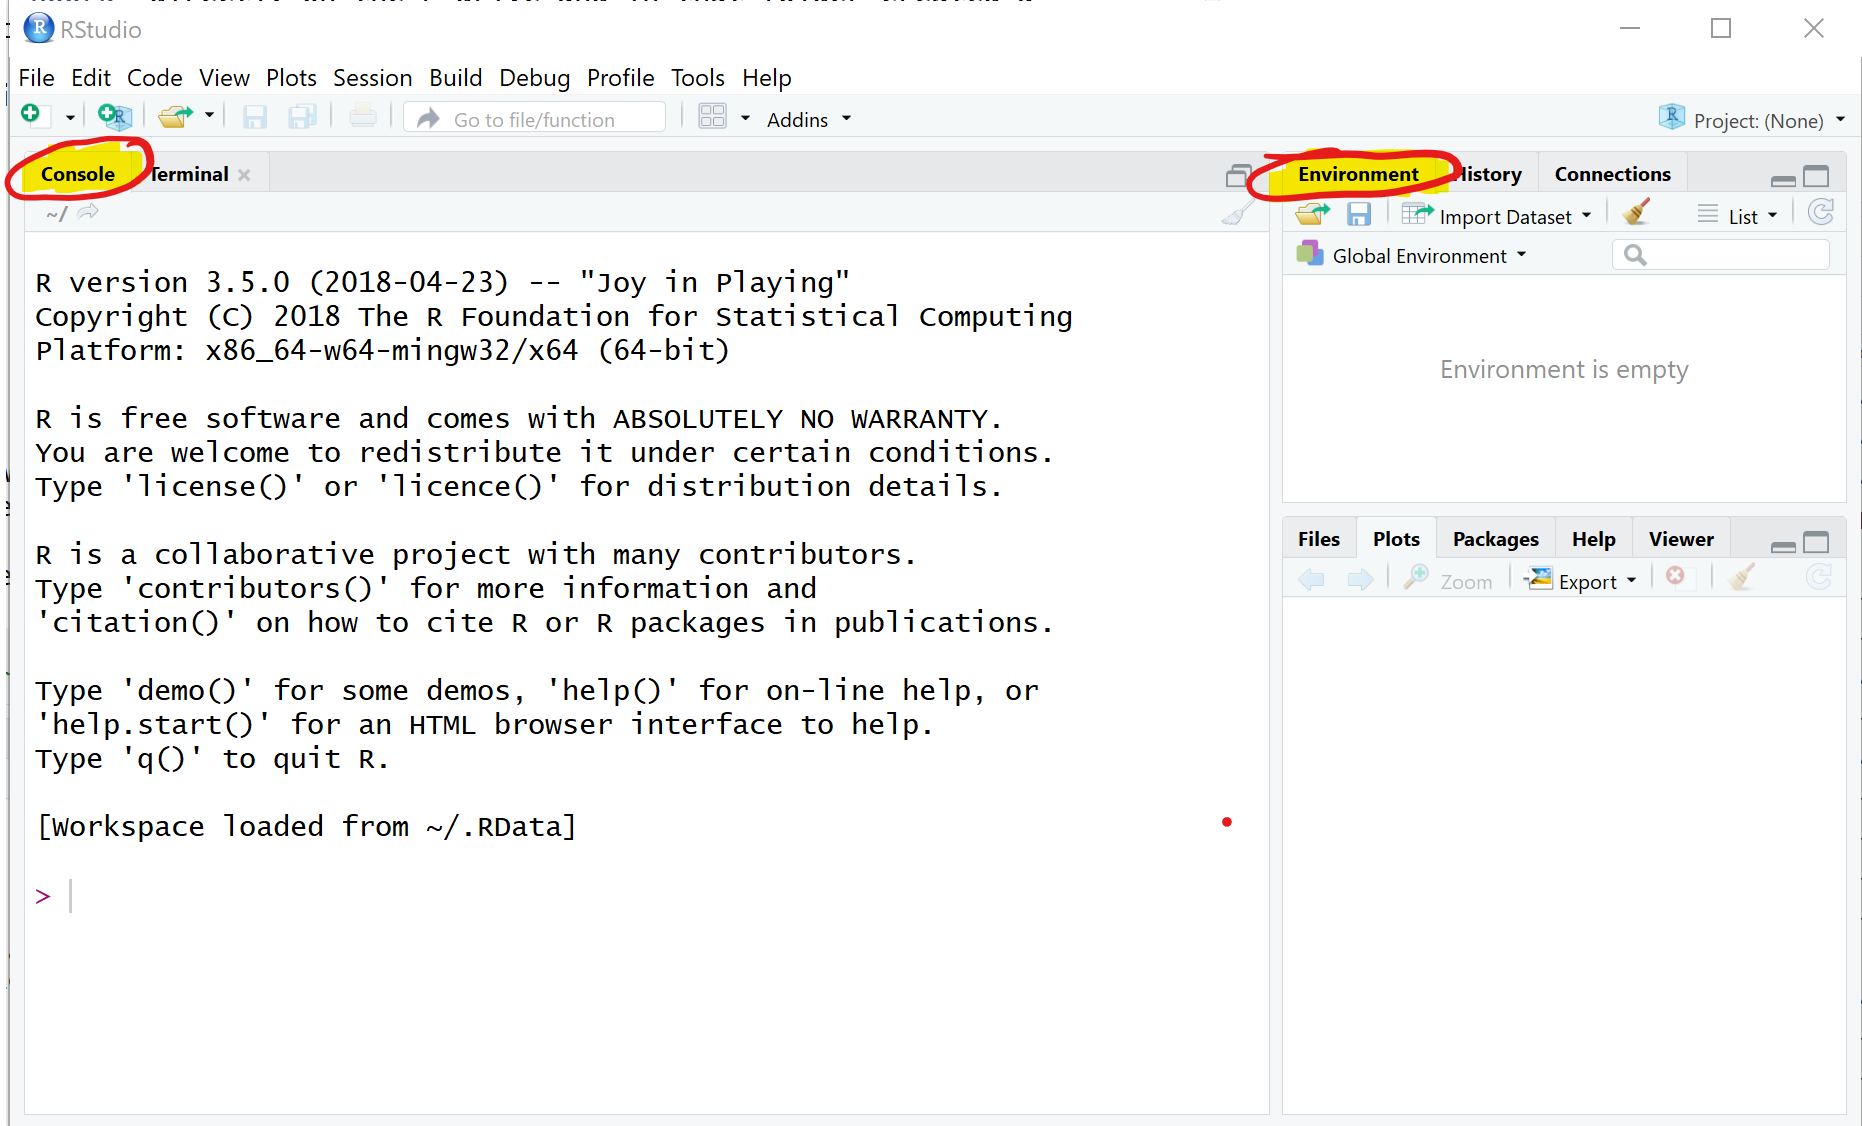
\includegraphics{RStudio_image0.png}
\caption{RStudio when loading for the first time}
\end{figure}

There are two important areas on that screen, the Console and the
Environment. The Console is something like your main computational area.
In there you can see some information but at the end an
``\textgreater{}''. This indicates that RStudio is standing ready to do
whatever you want it to do.

Say you want to calculate 3+4 \ldots{} yes, trivial but let's start
small. Type 3+4 into the console (behind the ``\textgreater{}'' sign and
press enter). Yes you should see the correct result.

\begin{Shaded}
\begin{Highlighting}[]
\DecValTok{3}\SpecialCharTok{+}\DecValTok{4}
\end{Highlighting}
\end{Shaded}

\begin{verbatim}
## [1] 7
\end{verbatim}

That was easy, let's see whether you can get R to calculate \(13^2\),
\(\sqrt{7569}\), \(e^{5}\) and \(ln(5)\). The first you achieve as
follows:

\begin{Shaded}
\begin{Highlighting}[]
\DecValTok{13}\SpecialCharTok{\^{}}\DecValTok{2}
\end{Highlighting}
\end{Shaded}

\begin{verbatim}
## [1] 169
\end{verbatim}

What about the others. Well, at this stage we will introduce you to the
most important programming techique there is, searching on the Web (say
in Google, Bing, Baidu, ChatGPT or Google Bart)! For instance if you
want to know how to calculate a square root in R you may want to search
for ``how to calculate a square root in R'' and you should find the
appropriate advice. Practice your search technique to calculate the
above solutions. Check against your calculator.

\hypertarget{functions}{%
\section{Functions}\label{functions}}

Functions are important building blocks of any programming language. You
just used your first function. Hopefully you found out that the way to
calculate \(\sqrt{7569}\) was to type

\begin{Shaded}
\begin{Highlighting}[]
\FunctionTok{sqrt}\NormalTok{(}\DecValTok{7569}\NormalTok{)}
\end{Highlighting}
\end{Shaded}

\begin{verbatim}
## [1] 87
\end{verbatim}

Giving you the result 87. What you used here is a function, namely the
\texttt{sqrt} function which some clever programmer wrote in order to
calculate a square root. The anatomy of a function is
\texttt{function\_name(input)}. Think of a function as a drink machine.

\begin{figure}
\centering
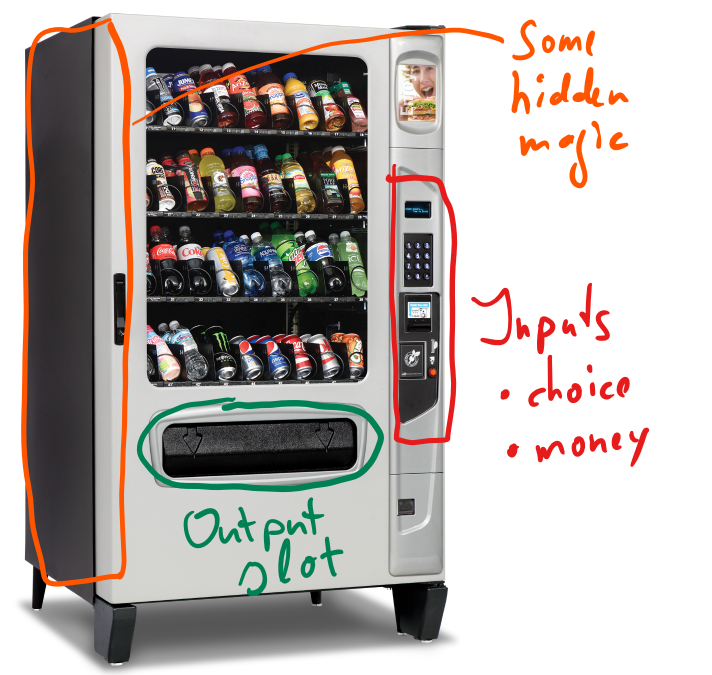
\includegraphics{DrinkMachine.png}
\caption{RStudio when loading for the first time}
\end{figure}

Most functions require some input. Our function, the \texttt{sqrt}
function needs a number of which to take the square root. The output in
our example, 87, is then returned. In our case it is returned to be
printed in the Console window.

\begin{quote}
Extension: If you feel that so far there was nothing new, you can try
and find out how to write your own functions in R. (If any of the above
was new to you then ignore this extension!!!)
\end{quote}

\hypertarget{creating-variables}{%
\section{Creating variables}\label{creating-variables}}

So far you have learned that R can be used as a glorified calculator.
Let's start to explore why R is way more powerful than that. You can
save the results of as many calculations as you want and you can easily
reuse the results of some calculations in later calculations.

Type ``a\textless-12/3'' into the console (without the quotation marks)
and press enter

\begin{Shaded}
\begin{Highlighting}[]
\NormalTok{a }\OtherTok{\textless{}{-}} \DecValTok{12}\SpecialCharTok{/}\DecValTok{4}
\end{Highlighting}
\end{Shaded}

You will see that in the console the correct result does not show, but
in the Environment pane of your RStudio window you should now see an
entry

\begin{figure}
\centering
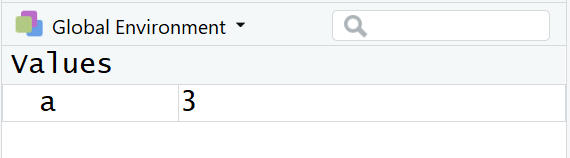
\includegraphics{RStudio_Env.png}
\caption{RStudio Environment saves variables}
\end{figure}

What did the command ``a\textless-12/4'' actually do? In words:
``Calculate 12/4 and assign (\textless-) the result to a variable called
\texttt{a}.''

With that in mind implement the following: ``Calculate 11*11 and assign
(\textless-) the result to a variable called \texttt{A}.''

You should now see two variables in your Environment pane. Let's add
another: ``Calculate the square root of 64 and assign (\textless-) the
result to a variable called \texttt{b}.''

Note that we used the \texttt{sqrt} function again, but this time the
output was not send to be printed in the Console, but instead it was
send to the new variable \texttt{b}. If you have done everything right
your Environment panel should now look as follows

\begin{figure}
\centering
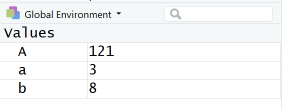
\includegraphics{RStudio_Env2.png}
\caption{RStudio Environment saves variables}
\end{figure}

Note that \texttt{a} and \texttt{A} are different variables, so R is
case-sensitive! All the variables listed in the Environment can be
re-used for further calculations. For example:

\begin{Shaded}
\begin{Highlighting}[]
\NormalTok{d }\OtherTok{\textless{}{-}}\NormalTok{ A }\SpecialCharTok{{-}}\NormalTok{ a }\SpecialCharTok{+} \DecValTok{2}\SpecialCharTok{*}\NormalTok{b}
\end{Highlighting}
\end{Shaded}

Let's perform another calculation in which we use the result of the last
calculation:

\begin{Shaded}
\begin{Highlighting}[]
\NormalTok{e }\OtherTok{\textless{}{-}}\NormalTok{ D }\SpecialCharTok{{-}} \DecValTok{3}\SpecialCharTok{*}\NormalTok{a}
\end{Highlighting}
\end{Shaded}

\begin{verbatim}
## Error in D - 3 * a: non-numeric argument to binary operator
\end{verbatim}

You will see R throwing an error message at you: ``Error in D - 3 * a :
non-numeric argument to binary operator''. Ehmmm \ldots{} what does this
mean? Actually not a lot. In the first instance this tells you that
something went wrong in that command. Can you see what the problem is?
Remember R is trying to perform the calculation to the right of
\texttt{\textless{}-} and then assign this to a new variable \texttt{e}.
Does it have all the info on the right hand side? Check your list of
variables in the Environment panel. Recall that R is case sensitive.

An important lesson with respect to error messages

\begin{itemize}
\tightlist
\item
  You will see them ALL THE TIME, and that is fine
\item
  You cannot break the computer with any errors in R, so don't worry,
  just try.
\item
  Re-read what you typed, is it actually what you wanted to do.
\item
  Read the error message. Sometimes it will give you a clue as to what
  the problem is \ldots{} unfortunately not here!
\end{itemize}

So, we have done a bit of work so far. Let's take a short break. Please
close RStudio and click ``Don't Save'' when you get the following
message

\begin{figure}
\centering
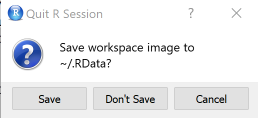
\includegraphics{RStudio_SaveWorkspace.png}
\caption{RStudio Environment saves variables}
\end{figure}

Get up, stretch your legs and get yourself a glass to drink. Then come
back and open RStudio again so that we can continue our work.

As you open you should get exactly the same initial layout as before
\ldots{} What value did \texttt{e} have again???? (125 if you managed to
correct the above error) Where are our calculations???

\hypertarget{preparing-your-script-file-and-libraries}{%
\section{Preparing your script file and
libraries}\label{preparing-your-script-file-and-libraries}}

For all significant work you want to make sure that you save the work
you have done, such that you do not have to re-type things which you did
yesterday \ldots{} or just before I asked you to get a glass of water.
The way to ensure that is to save all your work in a script file. A
script file is basically a text file which saves all your commands (and
comments - see below) and from where RStudio can easily execute these
commands.

Let's create a script file. Via the RStudio menu (FILE - NEW FILE - R
SCRIPT) open a new script file and save it in the folder from which you
want to work (see above).

Start by creating a comment line at the top of that file which may say
something like

\begin{Shaded}
\begin{Highlighting}[]
\CommentTok{\# File for first QM Computer Lab}
\CommentTok{\# February 2024}
\end{Highlighting}
\end{Shaded}

\begin{quote}
Note: Adding comments to your code is absolutely vital if you want to
understand tomorrow what you did today. I am not joking, adding comments
to explain to your future self what you are doing is absolutly critical.
Everything which follows the \texttt{\#} sign is a comment and is
effectively ignored by R. It is written not for R but for your future
self!
\end{quote}

If not mentioned otherwise all the following code could be added to that
script file and executed from there. However, the commands were actually
not worth saving. Let's start doing some proper data work. Save this
script file and make sure you know where you save it as, next week, you
should be continuing to work on this. Best to save it in your
\texttt{Rwork/QM} folder.

Next you should ensure that you set the working directory to the
directory where your scriptfile and datafile is in. If your folder was
\texttt{P:\textbackslash{}Rwork\textbackslash{}QM} then the command
below should read \texttt{setwd("P:/Rwork/QM")}. Note that all backward
slashes (\texttt{\textbackslash{}}) have to be replaced by forward
slashes (\texttt{/}). Don't ask why, just accept ;-).

\begin{Shaded}
\begin{Highlighting}[]
\FunctionTok{setwd}\NormalTok{(}\StringTok{"XXXX:/XXXX"}\NormalTok{)   }\CommentTok{\# replace the XXXX with your drive and path}
\end{Highlighting}
\end{Shaded}

Load the libraries which we want to use.

\begin{Shaded}
\begin{Highlighting}[]
\FunctionTok{library}\NormalTok{(tidyverse)    }\CommentTok{\# for almost all data handling tasks}
\end{Highlighting}
\end{Shaded}

\begin{verbatim}
## -- Attaching core tidyverse packages ------------------------ tidyverse 2.0.0 --
## v dplyr     1.1.1     v readr     2.1.4
## v forcats   1.0.0     v stringr   1.5.0
## v ggplot2   3.4.2     v tibble    3.2.1
## v lubridate 1.9.2     v tidyr     1.3.0
## v purrr     1.0.1     
## -- Conflicts ------------------------------------------ tidyverse_conflicts() --
## x dplyr::filter() masks stats::filter()
## x dplyr::lag()    masks stats::lag()
## i Use the ]8;;http://conflicted.r-lib.org/conflicted package]8;; to force all conflicts to become errors
\end{verbatim}

\begin{Shaded}
\begin{Highlighting}[]
\FunctionTok{library}\NormalTok{(readxl)       }\CommentTok{\# to import Excel data}
\FunctionTok{library}\NormalTok{(ggplot2)      }\CommentTok{\# to produce nice graphiscs}
\FunctionTok{library}\NormalTok{(stargazer)    }\CommentTok{\# to produce nice results tables}
\end{Highlighting}
\end{Shaded}

\begin{verbatim}
## 
## Please cite as: 
## 
##  Hlavac, Marek (2022). stargazer: Well-Formatted Regression and Summary Statistics Tables.
##  R package version 5.2.3. https://CRAN.R-project.org/package=stargazer
\end{verbatim}

\begin{quote}
Note: Libraries are collections of functions which add great
functionality. They are not included in the base R installation and
hence need to be added to your computer (see installation advice for
packages below - this only has to be done once on each computer).
However, even once they are installed you need to make this new
functionality available to your code. This is what the \texttt{library}
functions do. This has to be done at the beginning of every script file
in which you want to use the respective functionality.
\end{quote}

By just typing these commands into the script file nothing is actually
happening. If you want R to execute any of the commands in your script
file you have to do one of the following:

\begin{figure}
\centering
\includegraphics{RStudio_Image1.png}
\caption{RStudio Environment saves variables}
\end{figure}

\begin{enumerate}
\def\labelenumi{\arabic{enumi}.}
\tightlist
\item
  Press the ``Source'' button, in which case R will execute all commands
  in the script file
\item
  Press the ``Run'' button, in which case R will run the command in
  which the curser currently is
\item
  Press the ``CTRL''+``ENTER'' on the keyboard (COMMAND + CTRL on a
  Mac), in which case R will run the command in which the curser
  currently is
\item
  Highlight several lines and press ``CTRL''+``ENTER'' on the keyboard
  (COMMAND + CTRL on a Mac), in which case R will run the commands in
  the highlighted lines
\end{enumerate}

If RStudio tells you that one or more of these libraries are not
installed then install these (not any others) on the machine you are
working from. For instance, if \texttt{stargazer} was not installed you
would receive an error message like ``Error in library(stargazer) :
there is no package called `stargazer'\,'', and in that case you should
run:

\begin{Shaded}
\begin{Highlighting}[]
\FunctionTok{install.packages}\NormalTok{(}\StringTok{"stargazer"}\NormalTok{)}
\end{Highlighting}
\end{Shaded}

You can run this straight from the command/console or you could instead
install the package via the packages tab on the right hand side.
\textbf{Do not do this on computer lab computers as these packages
should be pre-installed}.

You will need to do this only once on your computer and once you have
done that you can call \texttt{library(stargazer)} again without running
into problems.

\hypertarget{data-upload}{%
\section{Data Upload}\label{data-upload}}

Make sure you have set the working directory to the directory in which
you saved your script file (see above). As we are dealing with data in
an excel file we will use the \texttt{read\_excel} function to load the
data.

Before you run the next command open the actual spreadsheet and try to
see how missing data are coded. In this case they are coded as dots
(``.''). But in other datafiles you may find ``NA'', ``n.a.'', ``-9999''
or other ways to code missing data. It is best to let R know how missing
data look. This will simplify your life tremendously.

\begin{Shaded}
\begin{Highlighting}[]
\NormalTok{CKdata }\OtherTok{\textless{}{-}} \FunctionTok{read\_excel}\NormalTok{(}\StringTok{"CK\_public.xlsx"}\NormalTok{,}\AttributeTok{na =} \StringTok{"."}\NormalTok{)}
\end{Highlighting}
\end{Shaded}

It is well possible that you receive the following error message as you
execute this command ``Error: \texttt{path} does not exist:
`CK\_public.xlsx'\,''. The most likely reason for this is that the
``CK\_public.xlsx'' is not saved in your working directory. Make sure
you download that file from Blackboard and save it in the working
directory you created earlier and you used in the \texttt{setwd()}
command.

Make sure that your data upload is successful. If you did you should see
an object \texttt{CKdata} in your environment. You can also run the
\texttt{str} (structure) function.

\begin{Shaded}
\begin{Highlighting}[]
\FunctionTok{str}\NormalTok{(CKdata)  }\CommentTok{\# prints some basic info on variables}
\end{Highlighting}
\end{Shaded}

\begin{verbatim}
## tibble [410 x 46] (S3: tbl_df/tbl/data.frame)
##  $ SHEET   : num [1:410] 46 49 506 56 61 62 445 451 455 458 ...
##  $ CHAIN   : num [1:410] 1 2 2 4 4 4 1 1 2 2 ...
##  $ CO_OWNED: num [1:410] 0 0 1 1 1 1 0 0 1 1 ...
##  $ STATE   : num [1:410] 0 0 0 0 0 0 0 0 0 0 ...
##  $ SOUTHJ  : num [1:410] 0 0 0 0 0 0 0 0 0 0 ...
##  $ CENTRALJ: num [1:410] 0 0 0 0 0 0 0 0 0 0 ...
##  $ NORTHJ  : num [1:410] 0 0 0 0 0 0 0 0 0 0 ...
##  $ PA1     : num [1:410] 1 1 1 1 1 1 0 0 0 1 ...
##  $ PA2     : num [1:410] 0 0 0 0 0 0 1 1 1 0 ...
##  $ SHORE   : num [1:410] 0 0 0 0 0 0 0 0 0 0 ...
##  $ NCALLS  : num [1:410] 0 0 0 0 0 2 0 0 0 2 ...
##  $ EMPFT   : num [1:410] 30 6.5 3 20 6 0 50 10 2 2 ...
##  $ EMPPT   : num [1:410] 15 6.5 7 20 26 31 35 17 8 10 ...
##  $ NMGRS   : num [1:410] 3 4 2 4 5 5 3 5 5 2 ...
##  $ WAGE_ST : num [1:410] NA NA NA 5 5.5 5 5 5 5.25 5 ...
##  $ INCTIME : num [1:410] 19 26 13 26 52 26 26 52 13 19 ...
##  $ FIRSTINC: num [1:410] NA NA 0.37 0.1 0.15 0.07 0.1 0.25 0.25 0.15 ...
##  $ BONUS   : num [1:410] 1 0 0 1 1 0 0 0 0 0 ...
##  $ PCTAFF  : num [1:410] NA NA 30 0 0 45 0 0 0 0 ...
##  $ MEALS   : num [1:410] 2 2 2 2 3 2 2 2 1 1 ...
##  $ OPEN    : num [1:410] 6.5 10 11 10 10 10 6 0 11 11 ...
##  $ HRSOPEN : num [1:410] 16.5 13 10 12 12 12 18 24 10 10 ...
##  $ PSODA   : num [1:410] 1.03 1.01 0.95 0.87 0.87 0.87 1.04 1.05 0.73 0.94 ...
##  $ PFRY    : num [1:410] 1.03 0.9 0.74 0.82 0.77 0.77 0.88 0.84 0.73 0.73 ...
##  $ PENTREE : num [1:410] 0.52 2.35 2.33 1.79 1.65 0.95 0.94 0.96 2.32 2.32 ...
##  $ NREGS   : num [1:410] 3 4 3 2 2 2 3 6 2 4 ...
##  $ NREGS11 : num [1:410] 3 3 3 2 2 2 3 4 2 4 ...
##  $ TYPE2   : num [1:410] 1 1 1 1 1 1 1 1 1 1 ...
##  $ STATUS2 : num [1:410] 1 1 1 1 1 1 1 1 1 1 ...
##  $ DATE2   : num [1:410] 111792 111292 111292 111492 111492 ...
##  $ NCALLS2 : num [1:410] 1 NA NA NA NA NA NA 2 NA 1 ...
##  $ EMPFT2  : num [1:410] 3.5 0 3 0 28 NA 15 26 3 2 ...
##  $ EMPPT2  : num [1:410] 35 15 7 36 3 NA 18 9 12 9 ...
##  $ NMGRS2  : num [1:410] 3 4 4 2 6 NA 5 6 2 2 ...
##  $ WAGE_ST2: num [1:410] 4.3 4.45 5 5.25 4.75 NA 4.75 5 5 5 ...
##  $ INCTIME2: num [1:410] 26 13 19 26 13 26 26 26 13 13 ...
##  $ FIRSTIN2: num [1:410] 0.08 0.05 0.25 0.15 0.15 NA 0.15 0.2 0.25 0.25 ...
##  $ SPECIAL2: num [1:410] 1 0 NA 0 0 0 0 0 0 0 ...
##  $ MEALS2  : num [1:410] 2 2 1 2 2 2 2 2 2 1 ...
##  $ OPEN2R  : num [1:410] 6.5 10 11 10 10 10 6 0 11 11 ...
##  $ HRSOPEN2: num [1:410] 16.5 13 11 12 12 12 18 24 11 10.5 ...
##  $ PSODA2  : num [1:410] 1.03 1.01 0.95 0.92 1.01 NA 1.04 1.11 0.94 0.9 ...
##  $ PFRY2   : num [1:410] NA 0.89 0.74 0.79 0.84 0.84 0.86 0.84 0.84 0.73 ...
##  $ PENTREE2: num [1:410] 0.94 2.35 2.33 0.87 0.95 1.79 0.94 0.94 2.32 2.32 ...
##  $ NREGS2  : num [1:410] 4 4 4 2 2 3 3 6 4 4 ...
##  $ NREGS112: num [1:410] 4 4 3 2 2 3 3 3 3 3 ...
\end{verbatim}

You should now see the \texttt{CKdata} object in your Environment (right
hand pane).

There are 410 observations, each representing one fast-food restaurant.
Each restaurant has some variables which characterise the store and then
two sets of variables which are observed before the new minimum wage was
introduced to New Jersey (Wave 1: Feb 15 to Mar 14, 1992) and after the
policy change (Wave 1: Nov 5 to Dec 31, 1992). Variables which relate to
the second wave will have a \texttt{2} at the end of the variable name.

The following variables will be important for the analysis here:

\begin{itemize}
\tightlist
\item
  \texttt{SHEET}, this is a unique identifier for each restaurant
\item
  \texttt{STATE}, 1 if New Jersey (NJ); 0 if Pennsylvania (Pa)
\item
  \texttt{WAGE\_ST}, starting wage (\$/hr), Wave 1
\item
  \texttt{WAGE\_ST2}, starting wage (\$/hr), after policy, Wave 2
\item
  \texttt{STATUS2}, the status of the Wave 2 interview, 0 = refused, 1 =
  completed, 3, permanently closed, 2, 4 and 5 = temporarily closed
\item
  \texttt{CHAIN}, 1 = Burger King; 2 = KFC; 3 = Roy Rogers; 4 = Wendy's
\item
  \texttt{EMPFT}, \# full-time employees before policy implementation
\item
  \texttt{EMPFT2}, \# full-time employees after policy implementation
\item
  \texttt{EMPPT}, \# part-time employees before policy implementation
\item
  \texttt{EMPPT2}, \# part-time employees after policy implementation
\item
  \texttt{NMGRS}, \# managers/ass't managers before policy
  implementation
\item
  \texttt{NMGRS2}, \# managers/ass't managers before policy
  implementation
\end{itemize}

You wrote your first script. It is time to have another break. Make sure
you save your script and the close RStudio (you don't need to do that in
general, but please do it at this point to help me demonstrate the value
of scripts). After relaxing for a few minutes and telling your flatmate
that you are on your way to become an expert programmer, come back and
re-open RStudio. Load the script file (if it wasn't loaded
automatically). The environment should, at this stage be empty, but if
you click on the ``Source'' button then R will automatically execute all
the commands you had in your script and \texttt{CKdata} should be
available in the Environment panel.

So that is the value of scripts! You can easily pick up where you left
your work, no need to redo anything.

\hypertarget{accessing-data}{%
\section{Accessing data}\label{accessing-data}}

The \texttt{CKdata} item in your environment basically contains the
entire spreadsheet of data. You can look at the entire spreadsheet by
clicking on the tiny spreadsheet in the \texttt{CKdata} line. This will
open a new tab with the spreadsheet. Have a look and then close the tab
again.

It is important to know how you can access subsets of data. Run through
the following commands to see what happens. Perhaps also experiment a
bit by changing the commands and predicting what the outcome should be.

\begin{Shaded}
\begin{Highlighting}[]
\NormalTok{CKdata[}\DecValTok{1}\NormalTok{,]}
\NormalTok{CKdata[,}\DecValTok{2}\NormalTok{]}
\NormalTok{CKdata[}\DecValTok{3}\NormalTok{,}\DecValTok{4}\NormalTok{]}
\NormalTok{CKdata[,}\DecValTok{4}\SpecialCharTok{:}\DecValTok{6}\NormalTok{]}
\NormalTok{CKdata[}\DecValTok{4}\SpecialCharTok{:}\DecValTok{6}\NormalTok{]}
\NormalTok{CKdata[}\DecValTok{2}\SpecialCharTok{:}\DecValTok{4}\NormalTok{,}\DecValTok{5}\SpecialCharTok{:}\DecValTok{10}\NormalTok{]}
\NormalTok{CKdata}\SpecialCharTok{$}\NormalTok{SOUTHJ}
\NormalTok{CKdata}\SpecialCharTok{$}\NormalTok{SOUTHJ[}\DecValTok{1}\SpecialCharTok{:}\DecValTok{5}\NormalTok{]}
\NormalTok{CKdata[}\FunctionTok{c}\NormalTok{(}\StringTok{"CHAIN"}\NormalTok{,}\StringTok{"STATE"}\NormalTok{)]}
\end{Highlighting}
\end{Shaded}

These are all different ways to select particular observations (rows in
a spreadsheet) and variables (columns in a spreadsheet). There were two
particular techniques which are important

\begin{itemize}
\tightlist
\item
  \texttt{CKdata\$CHAIN} did address the \texttt{CHAIN} variable in the
  \texttt{CKdata} dataset (\texttt{DATASET\$VARIABLE}).
\item
  \texttt{c("CHAIN","STATE")} allowed us to access two particular
  variables, ignoring all other 44 variables. It is useful to know what
  \texttt{c("CHAIN","STATE")} actually does.
\end{itemize}

\begin{Shaded}
\begin{Highlighting}[]
\FunctionTok{c}\NormalTok{(}\StringTok{"CHAIN"}\NormalTok{,}\StringTok{"STATE"}\NormalTok{)}
\end{Highlighting}
\end{Shaded}

\begin{verbatim}
## [1] "CHAIN" "STATE"
\end{verbatim}

It creates a list with two elements, here two text strings. But you can
also create lists with numbers.

\begin{Shaded}
\begin{Highlighting}[]
\FunctionTok{c}\NormalTok{(}\FloatTok{3.5}\NormalTok{,}\DecValTok{2}\SpecialCharTok{/}\DecValTok{3}\NormalTok{)}
\end{Highlighting}
\end{Shaded}

\begin{verbatim}
## [1] 3.5000000 0.6666667
\end{verbatim}

In fact you could even create lists which mixed datatypes.

\begin{Shaded}
\begin{Highlighting}[]
\FunctionTok{c}\NormalTok{(}\StringTok{"Countries in the EU"}\NormalTok{, }\DecValTok{28{-}1}\NormalTok{, }\StringTok{":{-}("}\NormalTok{)}
\end{Highlighting}
\end{Shaded}

\begin{verbatim}
## [1] "Countries in the EU" "27"                  ":-("
\end{verbatim}

Lists are quite fundamental to the way how R stores data. If you
assigned any of the above to a variable, for instance

\begin{Shaded}
\begin{Highlighting}[]
\NormalTok{silly\_list }\OtherTok{\textless{}{-}} \FunctionTok{c}\NormalTok{(}\StringTok{"Countries in the EU"}\NormalTok{, }\DecValTok{28{-}1}\NormalTok{, }\StringTok{":{-}("}\NormalTok{)}
\end{Highlighting}
\end{Shaded}

You would have saved it in the Environment and could re-use it.

All the commands in this section were really only to explore the
functionality of R. There is no need to save these in your script file.
But no harm either as none of these actually changed the values of the
data in \texttt{CKdata}.

\hypertarget{data-types}{%
\section{Data Types}\label{data-types}}

We can see (from the output to \texttt{str(CKdata)}) that all variables
are numeric (\texttt{num}) variables, i.e.~the software will treat them
as numbers. R did so, as we told it to treat ``.'' as missing values. If
you hadn't done so, it would have recognised a number of variables as
text variables (\texttt{chr}) which would not have been very helpful.

If you check the \texttt{CK\_codebook.txt} on BB you will find what all
the numbers mean. For instance an entry of \texttt{2} in the
\texttt{CHAIN} variable means that this is a ``KFC'' restaurant.

For later it will be convenient to have \texttt{STATE} and
\texttt{CHAIN} variables which aren't numeric, but categorical
variables. In R these are called \texttt{factor} variables. Hence we
will create two new variables, \texttt{STATEf} and \texttt{CHAINf} which
contain the same info, but just in a way easier to understand.

\begin{Shaded}
\begin{Highlighting}[]
\NormalTok{CKdata}\SpecialCharTok{$}\NormalTok{STATEf }\OtherTok{\textless{}{-}} \FunctionTok{as.factor}\NormalTok{(CKdata}\SpecialCharTok{$}\NormalTok{STATE)  }\CommentTok{\# translates a variable into a factor variable}
\FunctionTok{levels}\NormalTok{(CKdata}\SpecialCharTok{$}\NormalTok{STATEf) }\OtherTok{\textless{}{-}} \FunctionTok{c}\NormalTok{(}\StringTok{"Pennsylvania"}\NormalTok{,}\StringTok{"New Jersey"}\NormalTok{) }\CommentTok{\# changes the names of the categories}
\end{Highlighting}
\end{Shaded}

There are a number of important elements in these two lines

\begin{itemize}
\tightlist
\item
  \texttt{CKdata\$STATEf\ \textless{}-} creates a new variable in the
  \texttt{CKdata} object, called \texttt{STATEf}. \texttt{\textless{}-}
  is called the assignment operator and it assigns some value to that
  new variable. It will assign whatever comes to the right hand side of
  \texttt{\textless{}-}
\item
  \texttt{as.factor()} is a function called \texttt{as.factor}. If you
  want to find out what a function does you can call the help function
  \texttt{?as.factor}. This one ensures that creates a variable as a
  factor (categorical) variable. But it requires an input (Whatever
  comes inside the parenthesis). Here we ask R to change the
  \texttt{num} variable \texttt{CKdata\$STATE} into a factor variable.
\item
  \texttt{levels(CKdata\$STATEf)\ \textless{}-\ c("Pennsylvania","New\ Jersey")}
  then changes the names of the levels (categories) into sensible names.
  Here we use again the assignment operator \texttt{\textless{}-}. The
  order matters, but we learn from the codebook that: ``1 if NJ; 0 if
  PA''. As \texttt{STATE} is a numerical variable it will order the
  categories in numerical order, 0 (PA) first and 1 (NJ) next. In doubt
  you will have to check that you have used the right ordering by
  comparing the \texttt{STATE} and \texttt{STATEf} variable.
\end{itemize}

Now create a new variable \texttt{CHAINf} which achieves the same for
the \texttt{CHAIN} variable. Replace the \texttt{XXXX} to make this code
work. You will have to check the codebook for the right ordering.

\begin{Shaded}
\begin{Highlighting}[]
\NormalTok{CKdata}\SpecialCharTok{$}\NormalTok{XXXX }\OtherTok{\textless{}{-}} \FunctionTok{as.factor}\NormalTok{(XXXX}\SpecialCharTok{$}\NormalTok{XXXX)  }
\FunctionTok{XXXX}\NormalTok{(CKdata}\SpecialCharTok{$}\NormalTok{CHAINf) XXXX }\FunctionTok{c}\NormalTok{(}\StringTok{"XXXX"}\NormalTok{,}\StringTok{"KFC"}\NormalTok{, }\StringTok{"XXXX"}\NormalTok{, }\StringTok{"Wendy\textquotesingle{}s"}\NormalTok{) }
\end{Highlighting}
\end{Shaded}

Confirm that you have added the new variables and that they are indeed
of the factor type.

Or to avoid such a long output

Make sure you save your script file and for next week's exercise you
will pick up from this point.

Just as reminder, you learned quite a lot today. You can do some basic
navigation in RStudio and some very basic data manipulation. We will
continue doing some more and important investigation next week.

\end{document}
